\chapter{Literature Review}

Associative memory systems are a type of artificial intelligence technology
that is used for storing and retrieving information based on patterns or
associations. They are commonly used in applications such as pattern
recognition, data storage, and information retrieval.

Spiking neural networks are a type of neural network that models the behaviour
of biological neurons by using spikes or pulses to encode and transmit
information. They are a relatively new type of neural network that has the
potential to improve the performance and efficiency of artificial intelligence
systems.
The use of spiking neural networks for building associative memory systems is a relatively new area of research that has only recently started to gain
attention. 

Technical\cite{base} writing is writing or drafting technical communication used in
technical and occupational fields\cite{india}, such as computer hardware and
software\cite{rpi}, engineering, chemistry, aeronautics, robotics,
finance\cite{japan}, medical, consumer electronics, biotechnology, and
forestry. Technical writing encompasses the largest sub-field in technical
communication. See figure \ref{net2} that shows the autonomous systems in
Internet.

\begin{figure}[h!]
	\centering
	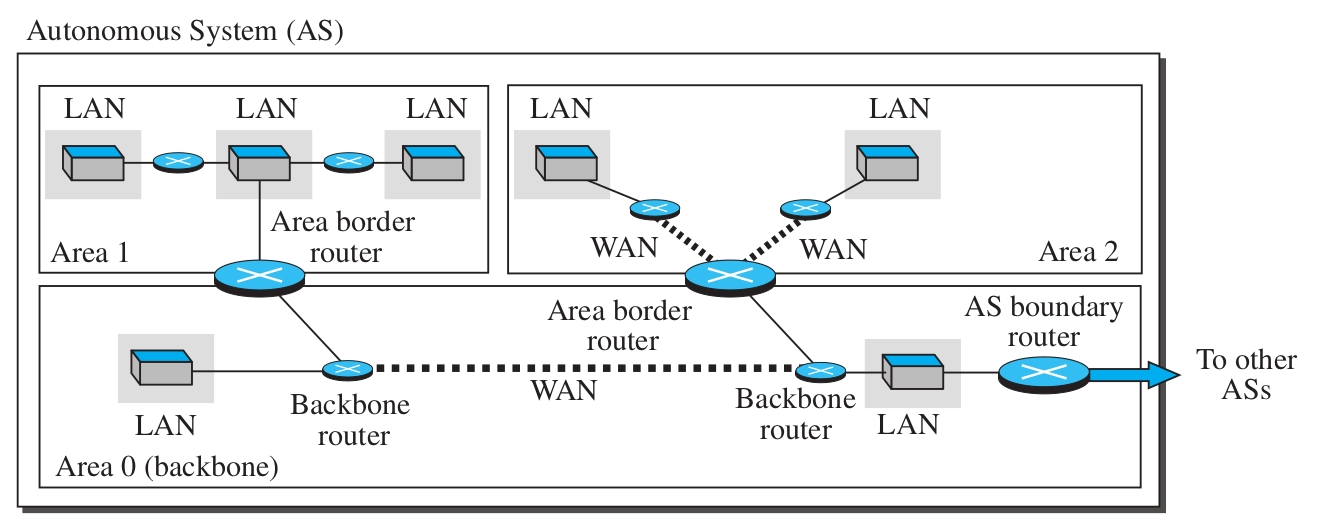
\includegraphics[width=0.9\linewidth]{ospf}
	\caption{Autonomous System Hierarchy}
	\label{net2}
\end{figure}

\section{section1}
\lipsum[2] % Please comment this line and type in the introduction chapter

\subsection{title 2}
\lipsum[3] % Please comment this line and type in the introduction chapter

\noindent The system is described by the equation \ref{sys_eq1} below. Here y is the ordinate and x is the abscissa , m is the slope and c a constant.

\begin{equation} \label{sys_eq1}
	y = mx + c
\end{equation}
\noindent Page centered and unnumbered multiple equations. The * symbol supresses equation numbering.
% Page centered and unnumbered equations
\begin{align*}
	2x - 5y & =  8   \\
	3x + 9y & =  -12
\end{align*}

\noindent Side by side figures can be created using this environment. See fig \ref{wave} below.
\begin{figure}[h!]
	\centering
	\begin{subfigure}[b]{0.4\textwidth}
		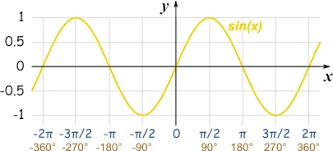
\includegraphics[width=\textwidth]{sinewave}
		\caption{Sine Wave}
		\label{fig:1}
	\end{subfigure}
	\hspace{20mm}
	\begin{subfigure}[b]{0.4\textwidth}
		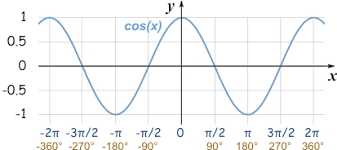
\includegraphics[width=\linewidth]{cosine}
		\caption{Cosine Wave}
		\label{fig:2}
	\end{subfigure}
	\caption{The Sine and Cosine waves}
	\label{wave}
\end{figure}